% ===== RUBRIC OF TEACHER'S JOB ASPECTS =====

% A single rubric criterion
\newcommand{\rubriccriterion}[4]{
\stepcounter{rubricquestion}
\section*{\therubricquestion: #1}

\smallskip
\note{Neznalý:} #2

\note{Začátečník:} #3

\note{Guru:} #4

\medskip
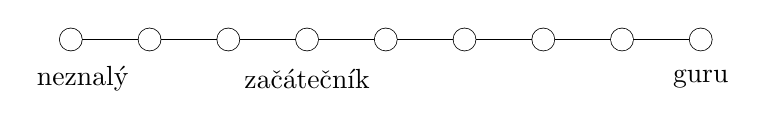
\begin{tikzpicture}
\draw (0,0) -- (8,0);
\foreach \i in {0,1,...,8} % numbers on line
{
\fill[black] (\i,0) circle (1.5 mm);
\fill[white] (\i,0) circle (1.4 mm);
}
\node at (0.15, -0.5) {neznalý};
\node at (3, -0.5)    {začátečník};
\node at (8, -0.5)    {guru};
\end{tikzpicture}
}

\restoregeometry
\chapter*{Učitelská rubrika}
\label{rubrika}

Na následujících stranách najdete rubriku činností učitele. Běžně si učitelé-začátečníci (a někdy ani učitelé-veteráni) neuvědomují možné úrovně a dimenze učitelské magie, prostě proto, že se s~nimi nikdy nepotkali. Je možné, že po pár měsících či letech učení přijde moment, kdy si uvědomíte, že máte mnohem větší prostor pro zlepšování, než jste si prve mysleli\punct{.}\footnote{Více informací najdete například v knize \emph{How Learning Works: Seven Research-Based Principles for Smart Teaching}.}

\section*{Co je to rubrika?}

Rubrika je nástroj pro \emph{self-assessment} (uvědomění a popsání svých vlastních znalostí a dovedností).
Pomáhá zřetelně si uvědomit a pojmenovat, jaké části daná věc má (např. umět programovat znamená být schopen navrhnout algoritmus, efektivně pracovat s~pamětí, znát syntaxi, \dots) a taky na jaké úrovni jsem já v jednotlivých částech (např. navrhnout algoritmus umím dobře, zapsat to kódem mám trochu problém a práci s pamětí neoptimalizuji vůbec).

\section*{Jak učitelskou rubriku používat?}

Na začátku semestru si rubriku vyplň (označ, kde na dané škále jsou podle tebe tvoje schopnosti). Vyber si 1--3 oblasti, na které se chceš zaměřit v tomto semestru a chceš-li být hodně důsledný(á), můžeš vymyslet i konkrétní kroky, které uděláš a indikátory svého postupu. Na konci semestru si můžeš rubriku vyplnit znovu a zhodnotit, v čem jsi se posunul(a).

Rubriku můžeš čist i jako manifest -- popisy kategorie \enquote{guru} vystihují naši představu o tom, co zvládají skvělí učitelé a co bychom rádi mezi cvičícími na fakultě kultivovali.

\newcounter{rubricquestion}

\newpage
\rubriccriterion{Vědomá pozornost a rozhodování, \textit{tracking}}
{Nedokážu si při výuce ani po ní vybavit, co se děje a jaký mám záměr. Při výuce se často cítím ztraceně.}
{Někdy se mi daří uvědomovat si, jaký mám právě záměr, co právě dělám a jaký to bude mít efekt. Většinou ale nemám při výuce vědomou pozornost.}
{Během výuky jsem si téměř vždy vědom(a) toho, co se se mnou i se skupinou děje, co dělám a jaký to bude mít efekt, kam směřuji. Dokážu si vybavit, jak jsme se dostali tam, kde právě jsme.}

\rule{\textwidth}{0.4pt}
\rubriccriterion{Interakce se skupinou, kladení otázek skupině}
{Se skupinou neinteraguji. Neptám se, asi bych nedostal(a) odpověď. Nevím, jak studenty dobře zapojit.}
{Vím, že lze interagovat se skupinou a znám nástroje (chápu, jak by to šlo). Nedokážu je ale často používat. Někdy  se skupiny ptám, ale nedostávám odpověď.}
{Se skupinou často a efektivně interaguji, ptám se způsobem, který studenty aktivizuje a zapojuje. Situace, kdy nedostávám ze skupiny odpověď dokážu obratně řešit (např. přeformulováním otázky).}

\newpage
\rubriccriterion{Strukturování výuky}
{O strukturování výuky nijak nepřemýšlím.}
{Chápu smysl přehledného strukturování své hodiny a snažím se o to. Často se ale zamotám, ztratím nit, nebo řeším mnoho naráz a studenti se pak ztrácí nebo odpojují.}
{Moje hodiny mají jasnou strukturu. Studenti ví, co se právě děje, co bude následovat a chápou návaznosti. Mezi jednotlivými bloky vědomě dělám zřetelné přechody.}

\rule{\textwidth}{0.4pt}
\rubriccriterion{Vlastní pocit z výuky}
{Svou výuku nijak nereflektuji.}
{Ve výuce si často moc nevěřím, vyžaduje to hodně energie, nebo se cítím napjatě. Mám strach z toho, na co se studenti zeptají.}
{Ve výuce se většinou cítím uvolněně a sebevědomě, mám svůj styl a baví mě to.}

\newpage
\rubriccriterion{Formativní zpětná vazba}
{O dávání zpětné vazby studentům nijak nepřemýšlím.}
{Snažím se studentům zpětnou vazbu dávat. Myslím si však, že jí není dost, nebo to nedělám efektivně, nebo to studenti nevnímají jako podporu a projev respektu.}
{Se studenty ve výuce interaguji tak, že dostávají průběžně formativní zpětnou vazbu. Chápou tedy, co jim jde, kde dělají chyby a jak se mohou zlepšovat. Zároveň se moji studenti cítí být respektováni a zpětné vazby se nebojí.}

\rule{\textwidth}{0.4pt}
\rubriccriterion{Jasné zadávání úloh}
{O zadávání úloh nijak zvlášť nepřemýšlím.}
{Stává se mi, že zadám úlohu a studenti neví, co dělat, jak začít nebo k čemu mají dojít (co má být výsledkem).}
{Když zadávám úlohu nebo aktivitu, mají studenti jasno v tom, co mají dělat a neřeší tak zbytečně věci, které nemám záměr procvičovat.}

\newpage
\rubriccriterion{Design výuky a variabilita aktivit}
{Učím tak, jak mi řekli nebo kopíruji výuku, kterou jsem viděl(a). Nepřemýšlím o~jiných variantách.}
{Jsem si vědom(a) toho, že existuje mnoho typů aktivit, které lze při výuce použít. Neznám jich ale dostatek, nedokážu je efektivně zadávat, nebo nemám jasno v tom, proč je vybírat.}
{Znám dostatek typů aktivit, svou výuku skládám tak, aby byla dostatečně pestrá. Vybrané aktivity efektivně učí/procvičují to, co mám záměr učit/procvičovat. Vybrané aktivity zároveň studenty efektivně zapojují a přispívají k jejich motivaci.}

\rule{\textwidth}{0.4pt}
\rubriccriterion{Širší kontext výuky a konkrétní hodiny}
{O širším kontextu výuky nepřemýšlím.}
{Uvědomuji si, že nemám pro sebe pojmenované znalosti a dovednosti, které u~studentů rozvíjím. Nevím, jak jejich pokrok sledovat. Nevím, v jakém kontextu to studenti využijí.}
{Mám jasnou představu o tom, k čemu studenty vedu, jaké dovednosti rozvíjím, jaké znalosti jim chci předat. Vím, proč tyto dovednosti rozvíjím a v jakém kontextu je studenti v budoucnu použijí. Vím, jak jejich pokrok sledovat.}
\vspace*{-1em}

\newpage
\rubriccriterion{Jasné vysvětlování}
{Svoje vysvětlování nijak nereflektuji.}
{Když vysvětluji, běžně se mi stává, že si nejsem jistý, zda vysvětluji dobře a zda to studentům pomáhá při pochopení.}
{Když vysvětluji teorii, demonstruji řešení nebo opravuji chybný postup. Dělám to efektivně a dokážu se dobře vžít do toho, jak to vidí student. Nestává se mi, že by studenti moje vysvětlení nechápali, nebo že bych vysvětloval(a) něco, na co se neptali.}

\rule{\textwidth}{0.4pt}
\rubriccriterion{Nastavení prostředí, systémy ve výuce}
{O nastavení atmosféry nepřemýšlím, systémy ve své výuce nevnímám.}
{Přemýšlím o nastavení pravidel i atmosféry. Systémy ve výuce (např. bodování) přebírám od ostatních. Nemám ale jasno v efektech, nebo neznám způsoby, jak je lze upravit.}
{Umím ve výuce vytvořit prostředí, které podporuje efektivní učení. U systémů, které používám (např. bodování, bonbóny, zahajovací rituály) chápu efekt. Systémy nepřebírám slepě, chápu jejich účel a uzpůsobuji podle svých potřeb.}

\newpage
\rubriccriterion{Improvizace, přizpůsobování}
{V průběhu své výuky na vzniklé situace nijak vědomě nereaguji.}
{Uvědomuji si chvíle, kdy by mohlo být zajímavé nebo užitečné dělat něco jiného, než jsem měl(a) v plánu. Většinou ale nedokážu v daný moment vhodně zareagovat.}
{Dokážu svoji výuku průběžně přizpůsobovat tomu, co se právě děje ve skupině a co studenti potřebují. Mám k tomu dostatek nástrojů a dokážu je efektivně použít.}

\rule{\textwidth}{0.4pt}
\rubriccriterion{Individuální interakce se studenty}
{O konzultacích nijak vědomě nepřemýšlím.}
{Stává se mi, že si nevím rady při individuální interakci se studentem (např. u~tabule, konzultace). Interakce neprobíhá efektivně nebo se student cítí zastrašen.}
{Při interakcích s jednotlivci (např. u tabule, konzultace) efektivně využívám čas. Studenti se mnou konzultují rádi, cítí ze mě respekt a podporu.}

\newpage
\rubriccriterion{Management skupiny, \textit{subgrouping}}
{Přijde mi, že dělit skupinu je zbytečnost, o~práci v~menších skupinkách nepřemýšlím.}
{Uvědomuji si možnosti práce ve dvojicích či menších skupinách. Tuším, že bych toho mohl(a) lépe využívat, hledám jak.}
{Mám jasno v tom, kdy chci pracovat se skupinou jako celkem, kdy s jednotlivci a kdy se skupinkami. Rozdělení do menších skupin efektivně používám. Ve vhodných případech zadávám interakce mezi skupinami.}

\rule{\textwidth}{0.4pt}
\rubriccriterion{Čtení skupiny}
{Skupinu ve své výuce nesleduji, pozornost věnuji pouze obsahu.}
{Uvědomuji si, že mi skupina vysílá signály a že by bylo dobré jim rozumět a využít je pro efektivní vedení výuky. Ve výuce to ale dokážu jen výjimečně.}
{Dokážu dobře odhadnout naladění skupiny. Mám jasno v tom, co se ve skupině studentů děje (např. únava, rezignace, zájem).}
